\section*{Question 1.3 - Sieve of Eratosthenes - MPI (Multi-Machine using MPI\_Reduce)}

In this question we were asked to rewrite our earlier implementation of the 
Sieve of Eratosthenes using MPI, while utilizing `MPI\_Bcast` and `MPI\_Reduce`. 
Once complete we were then asked to run the code on three server and note the 
speed-up/slow-down when compared to previous implementations.

\subsection*{Process}

\begin{itemize}
    \item We firstly removed any mentions of `MPI\_Send` and `MPI\_Recv` from our 
    implementation.
    \item We then refactored the code to use `MPI\_Bcast` and `MPI\_Reduce`
\end{itemize}

\subsection*{Difficulty}

When comparing to the our initial MPI implementation, using Broadcast and Reduce 
was far easier to write. However using OpenMP still far exceeds MPI in ease-of-use, 
readability and code-length.

\subsection*{Results}

\begin{figure}
    \centering
    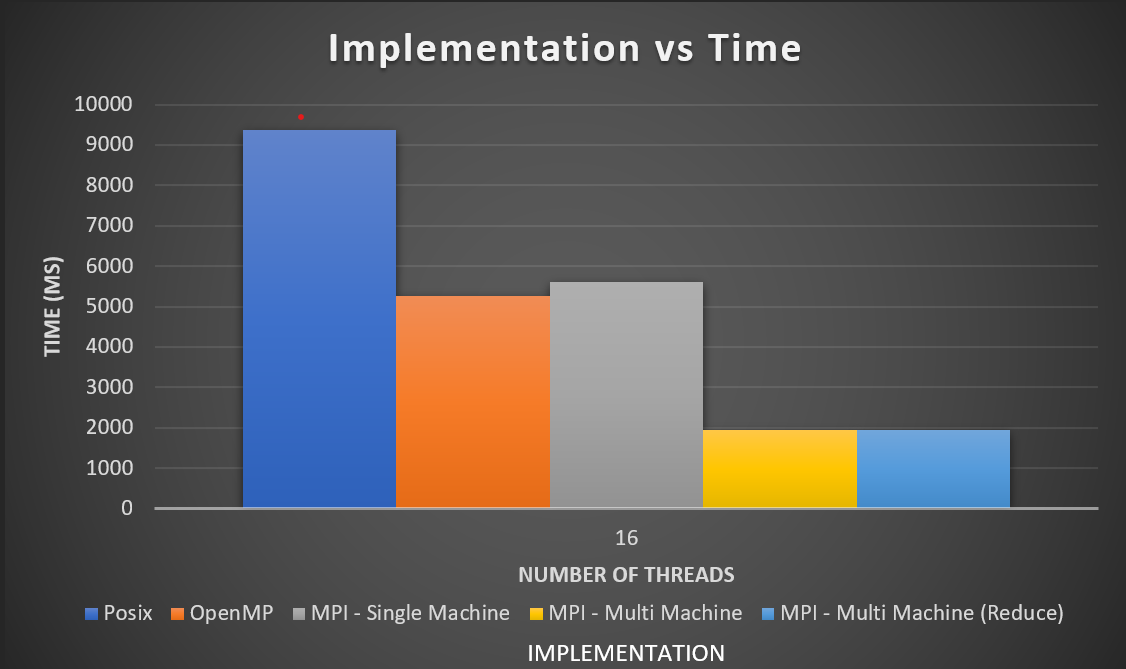
\includegraphics[width=\linewidth]{Figures/mpi_Bcast.png}
    \caption{Sieve of Eratosthenes with max number $9\times10^7$ on different
    implementations.}
    \label{fig:sievebcast}
\end{figure}

As seen in figure \ref{fig:sievebcast}, running the MPI implementation with `Broadcast` and 
`Reduce`, we see no noticeable slow-down or speed-up between the two 
implementations. This is most likely as our application does very little at 
send/receive or reduce time, therefore there would be no noticeable speed-up 
between the two algorithms. Therefore due to the slightly cleaner code and easier 
implementation, we would suggest using `MPI\_Bcast` and `MPI\_Reduce` to replace 
`MPI\_Send` and `MPI\_Recv` where possible.
